\documentclass[aspectratio=1610,14pt,t]{beamer}

% Colors
\usepackage{color}
\definecolor{mainorange}{HTML}{EC811B}
\definecolor{lightgrey}{HTML}{888888}

% Syntax highlighting
\usepackage{minted}
\usepackage{alltt}
\newcommand\hi[1]{{\color{mainorange} \textbf{#1}}}

% Custom unicode symbols
\usepackage{newunicodechar}
\newcommand\Warning{%
 \makebox[1.4em][c]{%
 \makebox[0pt][c]{\raisebox{.1em}{\small!}}%
 \makebox[0pt][c]{\color{red}\Large$\bigtriangleup$}}}%

\newunicodechar{⚠}{\Warning}

% Theme
\usetheme[%
	subsectionpage=progressbar,
	numbering=fraction,
	progressbar=foot,
]{metropolis}

% Customization
\setbeamertemplate{section in toc}[sections numbered]
\setbeamerfont{title}{size=\fontsize{30}{30}}
\setbeamerfont{block title}{size=\large}
\newcommand\sep{\textcolor{lightgrey}{\rule{\linewidth}{0.05mm}}}

% Positioning
% https://tex.stackexchange.com/a/34929/13059
\def\Put(#1,#2)#3{\leavevmode\makebox(0,0){\put(#1,#2){#3}}}

% Meta
\title{Calling Rust from C and Java}
\date{2017-10-31}
\author{Danilo Bargen (@dbrgn)}
\institute{Rust Zürichsee Meetup}

\begin{document}

\pgfdeclareimage[width=\paperwidth]{bg}{background-dark.pdf}
\usebackgroundtemplate{\pgfuseimage{bg}}
\maketitle

% ----------------------------------------------------------------- %

\begin{frame}[c]{println!("{:?}", Self)}
  Hi! I'm Danilo (@dbrgn).

  \pause

  I live in Rapperswil ({\small \texttt{instagram.com/visitrapperswil}}).

  \pause

  I work at Threema ({\small \texttt{threema.ch}}).

  \pause

  I'm a founding member of Coredump\\hackerspace ({\small \texttt{coredump.ch}}).
\end{frame}

% ----------------------------------------------------------------- %

\begin{frame}[plain,noframenumbering]
	\frametitle{Outline}
	\setcounter{tocdepth}{1}
	\tableofcontents
\end{frame}

% ----------------------------------------------------------------- %

\pgfdeclareimage[width=\paperwidth]{bg}{background-light.pdf}
\usebackgroundtemplate{\pgfuseimage{bg}}

\section{FFI}

\begin{frame}[c]{What is FFI?}
	FFI stands for <<Foreign Function Interface>>.

  It's a way to call functions written in one programming language
  from another one.
\end{frame}

\begin{frame}[c]{How does it work?}
  FFI works if there are known binary calling conventions that both sides adhere to.

  Think of it as a <<communication protocol>>.

  Not all languages have fixed calling conventions. C does, C++ does not.
\end{frame}

\begin{frame}[c]{FFI Is Easy!!!...?}
  Most FFI examples / intros do something like adding two integers.

  That is a totally useless example, since reality is much more complex.

  Biggest pain point once you get started: Heap allocations and pointers.
\end{frame}

\begin{frame}[c]{Memory Ownership}
  If you know Rust, you have probably acquired an intuitive understanding of the
  concept called <<Memory Ownership>>.

  The owner of an object owns its memory.
\end{frame}

\begin{frame}[c]{Let's Talk About Boxes}
  \centering
  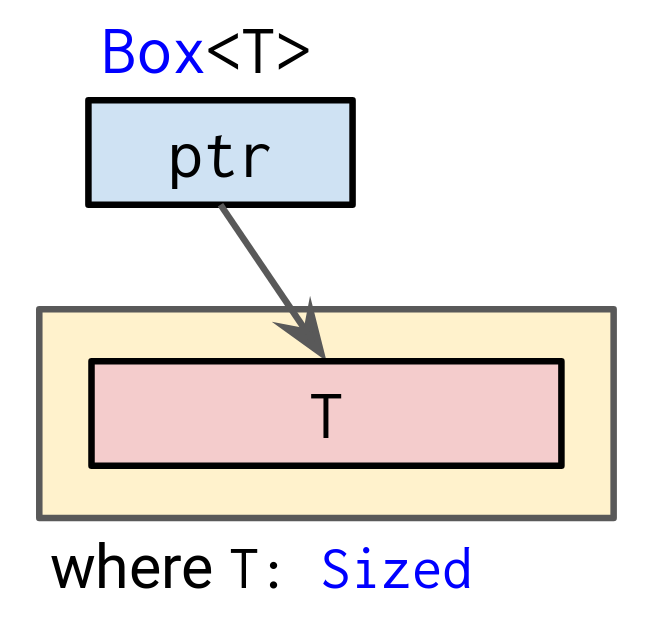
\includegraphics[width=.5\textwidth]{img/box.png}
\end{frame}

\begin{frame}[c]{Here Be Dragons}
    Rust ownership guarantees only cover memory allocated by Rust. For all
    other memory, we cannot make any assumptions.

  
\includegraphics[width=\textwidth]{img/dragons.jpg}
\end{frame}

\begin{frame}[c]{Rust: Beware the Drop}
  \begin{center}
  
\includegraphics[width=.5\textwidth]{img/dragon1.jpg}
  \end{center}

  When returning raw (unsafe) pointers from Rust, remember that the memory owned
  by Rust will be freed when the corresponding value is dropped.
\end{frame}

\begin{frame}[c]{C: Beware Other Allocators}
  \begin{center}
  
\includegraphics[width=.3\textwidth]{img/dragon2.jpg}
  \end{center}

  By default, Rust uses the jemalloc memory allocator and C does not.

  When handling memory allocated by Rust, do not try to free it in a C program.
\end{frame}

\begin{frame}[c]{Java: Beware the GC}
  \begin{center}
  
\includegraphics[width=.4\textwidth]{img/dragon3.jpg}
  \end{center}

  When holding on to a Java reference in Rust, the Java runtime must be notified
  about that. Otherwise the memory may be collected by the garbage collector.
\end{frame}

\begin{frame}[c]{It's Dangerous}
  \begin{center}
  
\includegraphics[width=.7\textwidth]{img/dangerous.png}

  \url{doc.rust-lang.org/nomicon/ffi.html}

  \url{jakegoulding.com/rust-ffi-omnibus/}

  \url{valgrind.org/}
  \end{center}
\end{frame}

% ----------------------------------------------------------------- %

\section{Parsing ICE Candidates}

\begin{frame}[c]{ICE Candidate Parsing}
  In order to have a practical example in this talk, we'll take a look at a
  simple library I've written.

  That library is a parser for ICE candidates with bindings for C and Java.

  Source: {\small \url{https://github.com/dbrgn/candidateparser}}
\end{frame}

\begin{frame}[c]{WTF are ICE Candidates?}
  \center
  
\includegraphics[width=.5\textwidth]{img/ice-skater.jpg}
\end{frame}

\begin{frame}[c]{WTF are ICE Candidates?}
  \begin{columns}[T]
    \begin{column}{.3\textwidth}
      
\includegraphics[width=\textwidth]{img/ice-skater.jpg}
    \end{column}
    \begin{column}{.7\textwidth}
      No, not that ice.

      \vspace{1em}

      \pause
      ICE stands for <<Interactive Connectivity Establishment>>.

      \vspace{1em}

      It's a protocol used in peer-to-peer networks to establish a connection.
    \end{column}
  \end{columns}
\end{frame}

\begin{frame}[c,fragile]{WTF are ICE Candidates?}
  This is what an ICE candidate looks like:

  \begin{minted}{rust}
candidate:842163049 1 udp 1686052607
1.2.3.4 46154 typ srflx
raddr 10.0.0.17 rport 46154 generation 0
ufrag EEtu network-id 3 network-cost 10
  \end{minted}
\end{frame}

\begin{frame}[c,fragile]{Parsing}
  Since this talk is about FFI, I won't cover the parsing in detail.

  The parser is written in Rust using
  nom\footnote{\url{https://crates.io/crates/nom}}.
  It provides a single function as entry point:

  \begin{minted}[fontsize=\small]{rust}
pub fn parse(sdp: &[u8]) -> Option<IceCandidate>
  \end{minted}
\end{frame}

\begin{frame}[c,fragile]{IceCandidate struct}

  This is the type returned by the parsing function:

  \begin{minted}[fontsize=\footnotesize]{rust}
pub struct IceCandidate {
    pub foundation: String,
    pub component_id: u32,
    pub transport: Transport,
    pub priority: u64,
    pub connection_address: IpAddr,
    pub port: u16,
    pub candidate_type: CandidateType,
    pub rel_addr: Option<IpAddr>,
    pub rel_port: Option<u16>,
    pub extensions: Option<HashMap<Vec<u8>, Vec<u8>>>,
}
  \end{minted}

  \Put(165, 360){
\includegraphics[height=1.4cm]{img/alloc.png}}
  \Put(175, 305){
\includegraphics[height=1.4cm]{img/unknown.png}}
  \Put(205, 250){
\includegraphics[height=1.4cm]{img/unknown.png}}
  \Put(220, 195){
\includegraphics[height=1.4cm]{img/unknown.png}}
  \Put(220, 165){
\includegraphics[height=1.4cm]{img/unknown.png}}
  \Put(310, 110){
\includegraphics[height=1.4cm]{img/alloc.png}}
\end{frame}

\begin{frame}[c,fragile]{Enums}
  Inside the \texttt{IceCandidate} struct, two enums are being used.

  \begin{minted}[fontsize=\small]{rust}
pub enum CandidateType {
  Host, Srflx, Prflx, Relay, Token(String)
}
  \end{minted}

  \begin{minted}[fontsize=\small]{rust}
pub enum Transport {
  Udp, Extension(String)
}
  \end{minted}

  Note that both of them contain associated data.

  \Put(275, 320){
\includegraphics[height=1.3cm]{img/alloc.png}}
  \Put(150, 200){
\includegraphics[height=1.3cm]{img/alloc.png}}
\end{frame}

\begin{frame}[c,fragile]{External Types}

  The \texttt{connection\_address} and the \texttt{rel\_addr} keys contain an
  \texttt{std::net::IpAddr}.

  \begin{minted}[fontsize=\small]{rust}
pub enum IpAddr {
    V4(Ipv4Addr),
    V6(Ipv6Addr),
}
  \end{minted}

  \Put(130, 155){
\includegraphics[height=1.3cm]{img/unknown.png}}
  \Put(130, 120){
\includegraphics[height=1.3cm]{img/unknown.png}}
\end{frame}

\begin{frame}[c,fragile]{Other Complex Types}

  The \texttt{extensions} key type:

  \vspace{3em}

  \texttt{Option<HashMap<Vec<u8>, Vec<u8>>>}.

  \Put(80, 110){
\includegraphics[height=1.3cm]{img/alloc.png}}
  \Put(140, 105){
\includegraphics[height=1.3cm]{img/alloc.png}}
  \Put(215, 105){
\includegraphics[height=1.3cm]{img/alloc.png}}
\end{frame}

% ----------------------------------------------------------------- %

\section{Rust $\rightleftharpoons$ C}

\begin{frame}[c]{Rust Types in C}

To be able to call Rust from C, we need to:

\begin{itemize}
  \item Make sure that all involved data types are \texttt{\#[repr(C)]}
  (simplifying Rust specific types)
  \pause
  \item Mark all exposed functions with \texttt{extern "C"} and
  \texttt{\#[no\_mangle]}
  \pause
  \item Compile the crate as a \texttt{cdylib}
\end{itemize}

\end{frame}

\begin{frame}[c]{Making Rust \#[repr(C)]}
  If we want to be able to call Rust from C, then all involved data types need
  to use C representation as memory layout.

  By default, the memory layout in Rust is unspecified. Rust is free to optimize
  and reorder fields.
\end{frame}

\begin{frame}[c,fragile]{IceCandidate: Rusty}
  \begin{minted}[fontsize=\small]{rust}
#[derive(Debug, PartialEq, Eq, Clone)]
pub struct IceCandidate {
    pub foundation: String,
    pub component_id: u32,
    pub transport: Transport,
    pub priority: u64,
    pub connection_address: IpAddr,
    pub port: u16,
    pub candidate_type: CandidateType,
    pub rel_addr: Option<IpAddr>,
    pub rel_port: Option<u16>,
    pub extensions: Option<HashMap<Vec<u8>, Vec<u8>>>,
}
  \end{minted}
\end{frame}

\begin{frame}[c,fragile]{IceCandidate: C-like}
  \begin{minted}[fontsize=\small]{rust}
#[repr(C)]
pub struct IceCandidateFFI {
    pub foundation: *const c_char,
    pub component_id: u32,
    pub transport: *const c_char,
    pub priority: u64,
    pub connection_address: *const c_char,
    pub port: u16,
    pub candidate_type: *const c_char,
    pub rel_addr: *const c_char, // Optional (nullptr)
    pub rel_port: u16, // Optional (0)
    pub extensions: KeyValueMap,
}
  \end{minted}
\end{frame}

\begin{frame}[c]{CStr and CString}
  There are two wrapper types to handle C strings:

  \begin{itemize}
    \item \texttt{std::ffi::CStr} (borrowed)
    \item \texttt{std::ffi::CString} (owned)
  \end{itemize}
\end{frame}

\begin{frame}[c,fragile]{String to *const c\_char}
  A Rust \texttt{String} can be converted to a \texttt{*const c\_char} through
  \texttt{CString}:

  \begin{minted}[fontsize=\small]{rust}
use std::ffi::CString;
use libc::c_char;

let s: String = "Hello".to_string();
let cs: CString = CString::new(s).unwrap();
let ptr: *const c_char = cs.into_raw();
  \end{minted}
\end{frame}

\begin{frame}[c,fragile]{String to *const c\_char}
  \begin{minted}[fontsize=\small]{rust}
let s: String = "Hello".to_string();
let cs: CString = CString::new(s).unwrap();
let ptr: *const c_char = cs.into_raw();
  \end{minted}

  ⚠ \textbf{Note:} \texttt{CString} is C compatible but should not be exposed
  directly through FFI!

  ⚠ \textbf{Note:} \texttt{CString::into\_raw()} transfers memory ownership to a
  C caller!
\end{frame}

\begin{frame}[c,fragile]{Custom types to *const c\_char}
  Our library generates some enums with associated data that cannot be
  represented directly as a C type. Return it as a C string instead!

  \begin{minted}[fontsize=\footnotesize]{rust}
pub enum Transport { Udp, Extension(String) }

impl Into<CString> for Transport {
    fn into(self) -> CString {
        match self {
            Transport::Udp => CString::new("udp").unwrap(),
            Transport::Extension(e) => CString::new(e).unwrap(),
        }
    }
}
  \end{minted}
\end{frame}

\begin{frame}[c,fragile]{Custom types to *const c\_char}
  We also return some external types like \texttt{IpAddr}. We cannot impl
  \texttt{Into<CString>} for those due to the orphan rule\footnote{You can write
  an impl only if either your crate defined the trait or defined one of the
  types the impl is for.}.

  Instead, convert them to a C string using the \texttt{ToString} trait!

  \begin{minted}[fontsize=\small]{rust}
let addr = CString::new(parsed.addr.to_string())
    .unwrap()
    .into_raw();
  \end{minted}
\end{frame}

\begin{frame}[c,fragile]{Optional types to C}
  C does not have a type directly corresponding to \texttt{Option<T>}. Instead,
  when dealing with heap allocated types, use (yuck!) null pointers.

  \begin{minted}[fontsize=\small]{rust}
let optional_ip = match parsed.rel_addr {
    Some(addr) => {
        CString::new(addr.to_string()).unwrap().into_raw()
    },
    None => std::ptr::null(),
}
  \end{minted}

  \pause

  For simpler types, use an "empty" value.

  \begin{minted}[fontsize=\small]{rust}
let optional_port = parsed.rel_port.unwrap_or(0);
  \end{minted}
\end{frame}

\begin{frame}[c]{HashMap to C}
  Now for some more complex types. Our \texttt{extensions} field has
  the type \texttt{Option<HashMap<Vec<u8>, Vec<u8>>>}.
\end{frame}

\begin{frame}[c]{Vec to C}
  Let's start with \texttt{Vec<T>}.

  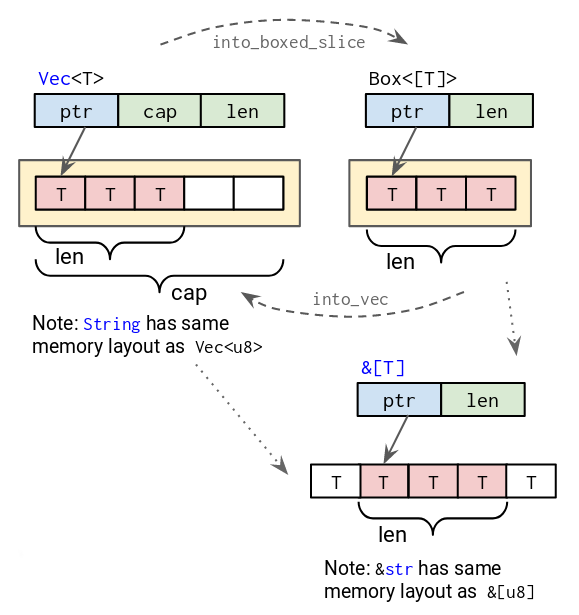
\includegraphics[width=.5\textwidth]{img/vec.png}
\end{frame}

\begin{frame}[c,fragile]{Vec to C: Option 1}
  Option 1: Shrink \texttt{Vec}, get a pointer, then forget the memory.

  \begin{minted}[fontsize=\small]{rust}
let mut v: Vec<u8> = vec![1, 2, 3, 4];
v.shrink_to_fit(); // assert_eq!(v.len(), v.capacity());
let ptr: *const uint8_t = v.as_ptr();
std::mem::forget(v);
  \end{minted}
\end{frame}

\begin{frame}[c,fragile]{Vec to C: Option 2}
  Option 2: Use \texttt{into\_boxed\_slice} and \texttt{into\_raw}.

  \begin{minted}[fontsize=\small]{rust}
let v: Vec<u8> = vec![1, 2, 3, 4];
let v_box: Box<[u8]> = v.into_boxed_slice();
let ptr: *const [uint8_t] = Box::into_raw(v_box);
  \end{minted}
\end{frame}

\begin{frame}[c,fragile]{Passing Vec to C}
  When passing a \texttt{Vec} to C, it is passed as a pointer to the first
  element.

  C needs to know how long our vector is!

  \begin{minted}[fontsize=\footnotesize]{rust}
let v: Vec<u8> = vec![1, 2, 3, 4];
let v_len: usize = v.len();
let v_ptr: Box<[u8]> = Box::into_raw(v.into_boxed_slice());
let raw_parts = (v_ptr, v_len);
  \end{minted}

  In C:

  \begin{minted}[fontsize=\footnotesize]{c}
for (size_t i = 0; i < rustvec.len; i++) {
    handle_byte(rustvec.ptr[i]);
}
  \end{minted}
\end{frame}

\begin{frame}[c,fragile]{Passing HashMap<Vec<u8>, Vec<u8>{}> to C}
  Pass a \texttt{HashMap} to C using a \texttt{KeyValuePair} type!

  \begin{minted}[fontsize=\footnotesize]{rust}
#[repr(C)]
pub struct KeyValuePair {
    pub key: *const uint8_t,
    pub key_len: size_t,
    pub val: *const uint8_t,
    pub val_len: size_t,
}

#[repr(C)]
pub struct KeyValueMap {
    pub values: *const KeyValuePair,
    pub len: size_t,
}
  \end{minted}
\end{frame}

\begin{frame}[c,fragile]{The Parsing Function}
  Phew! That was quite a lot. Now how do we actually expose this to C?

  ...using an \texttt{extern "C"} function.

  \begin{minted}[fontsize=\small]{rust}
#[no_mangle]
pub unsafe extern "C" fn parse_ice_candidate_sdp(
    sdp: *const c_char
) -> *const IceCandidateFFI {
  // ...
}
  \end{minted}
\end{frame}

\begin{frame}[c,fragile]{The Parsing Function: Reading C strings}
  Inside that function, we first need to convert the C char pointer to a Rust
  byte slice.

  \begin{minted}[fontsize=\small]{rust}
// `sdp` is a *const c_char
if sdp.is_null() {
    return std::ptr::null();
}
let cstr_sdp = CStr::from_ptr(sdp);
  \end{minted}

Note that we're using \texttt{CStr}, not \texttt{CString}!
\end{frame}

\begin{frame}[c,fragile]{The Parsing Function: Reading C strings}
Next, we parse the ICE candidate bytes using the regular Rust parsing function.

  \begin{minted}[fontsize=\small]{rust}
// Parse
let bytes = cstr_sdp.to_bytes();
let parsed: IceCandidate =
    match candidateparser::parse(bytes) {
        Some(candidate) => candidate,
        None => return ptr::null(),
    };
  \end{minted}
\end{frame}

\begin{frame}[c,fragile]{The Parsing Function: Reading C strings}
  Finally we convert the Rust type to the FFI type (using the techniques
  explained previously) and return a pointer to that.

  \begin{minted}[fontsize=\small]{rust}
// Convert to FFI representation
let ffi_candidate: IceCandidateFFI = ...;

// Return a pointer
Box::into_raw(Box::new(ffi_candidate))
  \end{minted}
\end{frame}

\begin{frame}[c,fragile]{Compiling as a C Library}
  To compile the Rust crate as a C compatible shared library, put this in your
  \texttt{Cargo.toml}:

  \begin{minted}[fontsize=\small]{rust}
[lib]
name = "candidateparser_ffi"
crate-type = ["cdylib"]
  \end{minted}

  This will result in a \texttt{candidateparser\_ffi.so} file.
\end{frame}

\begin{frame}[c]{Generating a Header File}
  To be able to use the library from C, you also need a header file.

  You can write such a header file by hand, or you can generate it at compile
  time using the \texttt{cbindgen} crate\footnote{\url{https://github.com/eqrion/cbindgen}}.

\end{frame}

\begin{frame}[c,fragile]{Calling the Parser from C}
  Include the header file and simply call the function:

  \begin{minted}[fontsize=\small]{c}
#include "candidateparser.h"
const IceCandidateFFI *candidate =
    parse_ice_candidate_sdp(sdp);
  \end{minted}

  Then link against the shared library when compiling:

  \begin{minted}[fontsize=\small]{bash}
$ clang example.c -o example \
    -L ../target/debug -l candidateparser_ffi \
    -Wall -Wextra -g
  \end{minted}

  A full example is available in the \texttt{candidateparser-ffi} crate on
  Github.
\end{frame}

\begin{frame}[c]{Cleaning up}
  Since we passed pointers from Rust to C, that memory cannot be freed by C!

  If we don't free it, we end up with memory leaks.

  We need to pass the pointers back to Rust to free the memory.
\end{frame}

\begin{frame}[c,fragile]{Cleaning up}

  First, create another function that accepts a pointer to an
  \texttt{IceCandidateFFI} struct.

  \begin{minted}[fontsize=\small]{rust}
#[no_mangle]
pub unsafe extern "C" fn free_ice_candidate(
    ptr: *const IceCandidateFFI
) {
    if ptr.is_null() { return; }
    // ...
}
  \end{minted}
\end{frame}

\begin{frame}[c,fragile]{Cleaning up}

  Now we create an owned \texttt{Box} from the pointer.

  \begin{minted}[fontsize=\small]{rust}
// Cast `*const T` to `*mut T`
let ptr: ptr as *mut IceCandidateFFI;

// Reconstruct box
let candidate: Box<IceCandidateFFI> = Box::from_raw(ptr);
  \end{minted}
\end{frame}

\begin{frame}[c,fragile]{Cleaning up Strings}

  Because the struct also contains pointers, we reconstruct Rust owned types
  from these pointers. The memory is freed as soon as those objects go out of
  scope!

  For strings:

  \begin{minted}[fontsize=\small]{rust}
CString::from_raw(candidate.foundation as *mut c_char);
  \end{minted}

  For nullable strings:

  \begin{minted}[fontsize=\small]{rust}
if !candidate.rel_addr.is_null() {
    CString::from_raw(candidate.rel_addr as *mut c_char);
}
  \end{minted}
\end{frame}

\begin{frame}[c,fragile]{Cleaning up Vec / KeyValueMap}

  Reclaiming the memory for our \texttt{KeyValueMap} is a bit more complex:

  \begin{minted}[fontsize=\footnotesize]{rust}
let e = candidate.extensions;
let pairs = Vec::from_raw_parts(e.values as *mut KeyValuePair,
                                e.len as usize, e.len as usize);
for p in pairs {
    Vec::from_raw_parts(p.key as *mut uint8_t, // Start
                        p.key_len as usize,    // Length
                        p.key_len as usize);   // Capacity
    Vec::from_raw_parts(p.val as *mut uint8_t, // Start
                        p.val_len as usize,    // Length
                        p.val_len as usize);   // Capacity
}
  \end{minted}
\end{frame}

\begin{frame}[c]{We Did It!}
  \centering
  Whew, that was a bumpy ride!

  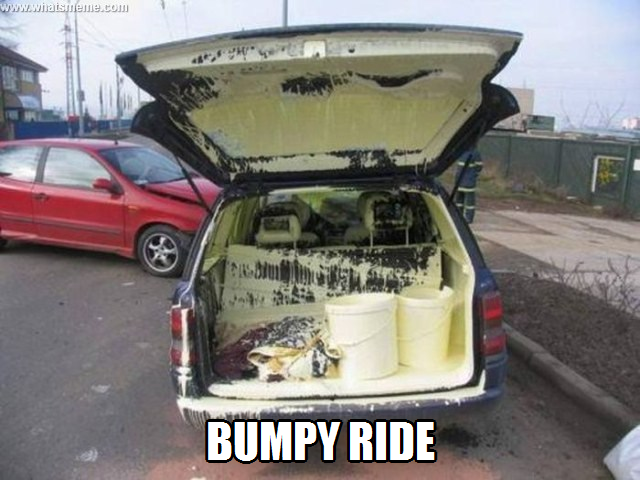
\includegraphics[width=.6\textwidth]{img/bump.png}
\end{frame}

% ----------------------------------------------------------------- %

\section{Rust $\rightleftharpoons$ Java}

\begin{frame}[c]{We Did It!}
  Ok, now for Java.

  Unfortunately we can't reuse the code we wrote for C.

  But we can reuse the concepts!
\end{frame}

\begin{frame}[c]{JNI}
  The "classic" way to talk to Java from external languages is through JNI (Java
  Native Interface).

  There are newer options by now (namely JNA), but as far as I know there are
  issues with that if you want to run your code on Android.
\end{frame}

\begin{frame}[c,fragile]{Preparations}
  First, we have to write classes for all Java types we're going to use. Since
  it's Java, it's a bit verbose.

  \begin{minted}[fontsize=\footnotesize]{java}
package ch.dbrgn.candidateparser;
import java.util.HashMap;

public class IceCandidate {
    // Non-null fields
    private String foundation;
    private long componentId;
    private String transport;
    private long priority;
    private String connectionAddress;
    private int port;
    private String candidateType;
  \end{minted}
\end{frame}

\begin{frame}[c,fragile]{Preparations}
  \begin{minted}[fontsize=\footnotesize]{java}
    // Extensions
    private HashMap<String, String> extensions = new HashMap<>();

    // Nullable fields
    private String relAddr = null;
    private Integer relPort = null;

    public IceCandidate(String foundation, long componentId,
                        String transport, long priority,
                        String connectionAddress, int port,
                        String candidateType) {
        this.foundation = foundation;
        this.componentId = componentId;
        // ...
    }

  \end{minted}
\end{frame}

\begin{frame}[c,fragile]{Preparations}
  Next, we'll write the "interface" for the parser class.

  \begin{minted}[fontsize=\footnotesize]{java}
package ch.dbrgn.candidateparser;

public class CandidateParser {
    static {
        System.loadLibrary("candidateparser_jni");
    }

    public static native IceCandidate parseSdp(String sdp);
}
  \end{minted}

Note the \texttt{native} modifier.
\end{frame}

\begin{frame}[c,fragile]{Generating JNI Headers}
  To generate the JNI headers, we first compile the \texttt{.java} files:

  \begin{minted}[fontsize=\footnotesize]{bash}
$ javac -classpath app/src/main/java/ \
    app/src/main/java/ch/dbrgn/candidateparser/IceCandidate.java
$ javac -classpath app/src/main/java/ \
    app/src/main/java/ch/dbrgn/candidateparser/CandidateParser.java
  \end{minted}

  Then use the \texttt{javah} tool to generate the JNI header.

  \begin{minted}[fontsize=\footnotesize]{bash}
$ javah -classpath app/src/main/java/ \
    -o CandidateParserJNI.h \
    ch.dbrgn.candidateparser.CandidateParser
  \end{minted}
\end{frame}

\begin{frame}[c,fragile]{Generating JNI Headers}
  The header file (minus some boilerplate):
  \begin{minted}[fontsize=\footnotesize]{c}
#include <jni.h>

/*
 * Class:     ch_dbrgn_candidateparser_CandidateParser
 * Method:    parseSdp
 * Signature: (Ljava/lang/String;)Lch/dbrgn/candidateparser
 *                                                     /IceCandidate;
 */
JNIEXPORT jobject JNICALL
  Java_ch_dbrgn_candidateparser_CandidateParser_parseSdp
  (JNIEnv *, jclass, jstring);
  \end{minted}

\end{frame}

\begin{frame}[c,fragile]{Rust Bindings for JNI}
  Create a new library and add the
  \texttt{jni}\footnote{\url{https://github.com/prevoty/jni-rs}} crate as
  dependency.

  \begin{minted}[fontsize=\small]{ini}
[dependencies]
jni = "0.6"

[lib]
crate_type = ["dylib"]
  \end{minted}

\end{frame}

\begin{frame}[c,fragile]{lib.rs}
  In \texttt{lib.rs}, create a function with the same name as the function in
  the JNI header.

  \begin{minted}[fontsize=\footnotesize]{rust}
#[no_mangle]
#[allow(non_snake_case)]
pub extern "system"
fn Java_ch_dbrgn_candidateparser_CandidateParser_parseSdp(
    env: JNIEnv,
    _class: JClass,
    input: JString)
    -> jobject {

    // ...

}
  \end{minted}

\end{frame}

\begin{frame}[c,fragile]{Converting parameters}
  To get a reference to a Java String we need to access it through the
  \texttt{JNIEnv} instance and convert it to a Rust \texttt{String}.

  \begin{minted}[fontsize=\footnotesize]{rust}
let sdp: String = env.get_string(input).unwrap().into();
  \end{minted}

  Now we can simply pass it to the regular Rust function!

  \begin{minted}[fontsize=\footnotesize]{rust}
let candidate = match candidateparser::parse(sdp.as_bytes()) {
    Some(cand) => cand,
    None => return std::ptr::null_mut() as *mut _jobject, // hack
};
  \end{minted}
\end{frame}

\begin{frame}[c,fragile]{Creating New Java Objects}

  Since we want to return the parsed candidate to Java, we want to instantiate
  the Java \texttt{IceCandidate} class.

  \begin{minted}[fontsize=\footnotesize]{rust}
let obj: JObject = env.new_object(
  // Classpath
  "ch/dbrgn/candidateparser/IceCandidate",
  // Signature
  "(Ljava/lang/String;JLjava/lang/String;J
    Ljava/lang/String;ILjava/lang/String;)V",
  // Argument slice containing `JValue`s
  &args
).unwrap();
  \end{minted}

  JNI signature syntax:\\
  {\footnotesize https://docs.oracle.com/javase/8/docs/technotes/guides/jni/spec/types.html}

\end{frame}

\begin{frame}[c,fragile]{Creating New Java Objects}
  The arguments need to be wrapped in JNI wrapper types. This makes sure that
  the JVM GC knows about them. Two examples:

  \begin{minted}[fontsize=\footnotesize]{rust}
let component_id = JValue::Long(candidate.component_id as jlong);

let foundation = JValue::Object(
    env.new_string(&candidate.foundation).unwrap().into()
);
  \end{minted}
\end{frame}

\begin{frame}[c,fragile]{Calling Java Functions}
  TODO
  \begin{minted}[fontsize=\footnotesize]{rust}
  \end{minted}
\end{frame}

% ----------------------------------------------------------------- %

\section{Questions?}

% ----------------------------------------------------------------- %

{
\setbeamertemplate{footline}{}
\pgfdeclareimage[width=\paperwidth]{bg}{background-inverted.pdf}
\usebackgroundtemplate{\pgfuseimage{bg}}
\begin{frame}[standout]
	\begin{centering}
	{\Huge Thank you!}\\
	{\normalsize \url{www.coredump.ch}}\\
	\end{centering}
\end{frame}
}

\end{document}
